\documentclass[10pt,twocolumn]{article}

% --- Packages (all standard; compiles on Overleaf with pdfLaTeX) ---
\usepackage[margin=0.85in]{geometry}
\usepackage{amsmath,amssymb}
\usepackage{booktabs}
\usepackage{graphicx}
\usepackage{xcolor}
\usepackage{listings}
\usepackage{microtype}
\usepackage{balance}
\usepackage{pgfplots}
\pgfplotsset{compat=1.16}
\usepackage[numbers,sort&compress]{natbib}
\usepackage[hidelinks]{hyperref}
\usepackage{cleveref}

% --- Single source of truth for measured numbers (from bench/results/) ---
% Apple M5, Qwen3-4B, Metal, greedy, median of 5 (decode 64) / 5 (prefill).
\newcommand{\DecodeBF}{12.6}
\newcommand{\DecodeQEight}{20.7}
\newcommand{\DecodeAffineFour}{26.9}
\newcommand{\PrefillBF}{143}
\newcommand{\PrefillQEight}{35}
\newcommand{\PrefillAffine}{32}
\newcommand{\PeakRSS}{41}
% Speculative decoding (bench/spec_bench.py + controlled A/B, Q8_0 4B, M5):
\newcommand{\SpecDecodeRep}{41.9}   % spec decode tok/s, repetitive (was 21.7)
\newcommand{\SpecSpeedupRep}{1.93}  % spec wall-clock speedup, repetitive
\newcommand{\SpecSpeedupCode}{0.88} % spec speedup, code (hurts)
\newcommand{\SpecSpeedupChat}{0.55} % spec speedup, open-ended (hurts most)

\lstset{basicstyle=\ttfamily\footnotesize,breaklines=true,frame=single,
        columns=fullflexible,keepspaces=true}
\newcommand{\code}[1]{\texttt{\small #1}}

\title{\textbf{Kipp: Oracle-Gated, Placement-Invariant Paged\\
Attention for Verifiable LLM Inference}}
\author{David Khachatryan Johansson\\ \small \texttt{david@cortify.io}}
\date{\today}

\begin{document}
\maketitle

\begin{abstract}
We introduce \textbf{Kipp}, a hand-written C11 inference engine for the pinned
Qwen3 dense model family with a scalar CPU reference oracle and
correctness-gated Apple~Metal and NVIDIA~CUDA backends. Modern serving systems
adopted \emph{paged} key--value (KV) caches to eliminate memory fragmentation,
and in doing so came to \emph{rely} on a subtle correctness property: that the
physical placement of KV blocks does not affect the model's output. That
property is universally assumed and never tested. Kipp turns it into a
machine-checked contract. Its paged-attention kernels are written to be
\emph{physical-placement invariant}, and a gate reverses (scrambles) each
sequence's block table and asserts the generated logits are
\emph{bitwise-identical} to the identity mapping---an adversarial test that
catches KV-addressing bugs which tolerance-based reference comparisons miss.
A deliberately scalar CPU oracle, held byte-stable across refactors, serves as
a \emph{hard} regression gate rather than a soft baseline: every GPU backend
must match it to identical arg\,max within $10^{-4}$ NMSE. On an Apple~M5, Kipp
decodes Qwen3-4B at \DecodeBF{}~tok/s in BF16, \DecodeQEight{}~tok/s at 8-bit,
and \DecodeAffineFour{}~tok/s at 4-bit, in $\sim$\PeakRSS{}~MB of resident
memory, and reaches \SpecDecodeRep{}~tok/s ($\SpecSpeedupRep\times$) on
copy-heavy text via prompt-lookup speculation that is token-identical to
greedy decoding. We do not claim to be the fastest engine; we claim an engine
whose paging, prefix reuse, and speculative rollback are correct by continuous
construction, and every number is reproducible by re-execution.
\end{abstract}

\section{Introduction}
\label{sec:intro}
Large language model (LLM) serving is dominated by the cost of the
key--value (KV) cache. \citet{kwon2023pagedattention} observed that reserving
a contiguous KV region per request wastes $60$--$80\%$ of KV memory to
internal and external fragmentation, and introduced \emph{PagedAttention}:
store KV in fixed-size blocks and give each sequence a \emph{block table}
mapping logical positions to arbitrary physical blocks, exactly as an
operating system pages virtual memory. Paging is now standard
\citep{kwon2023pagedattention,zheng2024sglang}; it underpins prefix sharing,
live block migration, and speculative-decode rollback.

Paging rests on an unstated assumption: \emph{where} a block physically lives
must not change \emph{what} the model computes. Systems that relocate KV
blocks at runtime---for load balancing \citep{kwon2023pagedattention}, cache
sharing \citep{zheng2024sglang}, or memory defragmentation---treat this
placement-invariance as safe by construction and never test it. Yet the
indirection it depends on (a per-access \code{block\_table[pos>>5]*32 +
(pos\&31)} lookup, replicated across every backend and kernel) is precisely
where off-by-one and stride bugs hide, and such bugs are \emph{silent}: they
corrupt a few positions without crashing, and a tolerance-based comparison to
a reference forward pass---the standard test---can mask them as numerical
noise.

Kipp takes the opposite stance. We make placement-invariance an explicit,
adversarially-tested \emph{contract}. Concretely, this paper contributes:

\begin{enumerate}\itemsep2pt
  \item \textbf{A placement-invariance gate} (\Cref{sec:vpa}): we reverse each
  sequence's block table and assert the output logits are \emph{bitwise}
  identical to the identity mapping. This is a cheap, backend-agnostic
  adversarial test for a class of paging bugs that reference comparisons miss,
  stated with the precise scope under which invariance holds.
  \item \textbf{An oracle-gated backend discipline} (\Cref{sec:oracle}): a
  scalar CPU forward pass, held byte-identical across the engine's evolution,
  is used as a \emph{hard} gate; Metal and CUDA must match it at identical
  arg\,max within $10^{-4}$ NMSE. This inverts the common assumption that
  optimized GPU kernels are ``never bitwise-equal'' to a reference.
  \item \textbf{A small, readable, verifiable engine} (\Cref{sec:impl,sec:eval}):
  $\sim$8\,k lines of C11 core (plus $\sim$3\,k for the Metal and CUDA
  backends) running the Qwen3 dense family across CPU, Metal, and CUDA, with
  8- and 4-bit quantization, continuous batching, an OpenAI-compatible server,
  and prompt-lookup speculation---at real, reproducible throughput, in tens of
  megabytes of RAM.
\end{enumerate}

We are explicit about what is \emph{not} new. Attention is invariant to a
permutation of stored KV under a matching permutation of the causal mask; this
is folklore and has been treated formally in recent KV-quantization work. Zero
memmove during speculative rollback is standard paged-cache behavior
\citep{leviathan2023speculative}. Our contribution is not the property but the
\emph{engineering discipline of testing it}, and the artifact that results.

\section{Background}
\label{sec:bg}
\paragraph{The Qwen3 dense family.} Kipp targets a fixed registry of pinned
Qwen3 dense checkpoints (0.6B--32B, base and instruct). The family shares
head dimension $128$, $8$ KV heads, vocabulary $151{,}936$, RMSNorm
$\epsilon=10^{-6}$, NEOX rotary embeddings, grouped-query attention, and
SwiGLU MLPs; only depth, width, head count, and rope~$\theta$ vary. Fixing the
family (rather than accepting arbitrary GGUF files) is what makes exact,
per-checkpoint validation tractable.

\paragraph{Paged KV cache.} A sequence's KV is stored in physical blocks of
$B{=}32$ positions. A per-sequence \emph{block table} $\pi$ maps logical block
$b$ to a physical block $\pi(b)$; position $p$ resolves to physical slot
$\pi(\lfloor p/B\rfloor)\cdot B + (p \bmod B)$. The identity table
$\pi(b){=}b$ reproduces a contiguous cache byte-for-byte. Prefix sharing, block
migration, and rollback are all realized by editing $\pi$, never by moving KV
bytes.

\section{Placement-Invariant Paged Attention}
\label{sec:vpa}
\paragraph{The property.} Let a sequence occupy logical positions
$0,\dots,L-1$. For any permutation $\pi$ of the physical blocks that is applied
consistently to both KV \emph{writes} and \emph{reads}, the attention output
for every query position is unchanged, because attention at position $p$ is a
mask-weighted reduction over the \emph{set} of source positions $\{0,\dots,p\}$
and each source's key/value is read from wherever $\pi$ placed it. Placement
enters only the address, never the value or the reduction order. Hence the
final logits are identical---and, since the reduction order is fixed,
\emph{bitwise} identical, not merely close.

\paragraph{Scope (stated precisely).} Invariance holds for the \emph{physical
placement of retained KV}: reordering which physical block holds a given
\emph{logical} position. It does \emph{not} hold for reordering the logical
positions themselves---rotary embeddings and the causal mask are
position-dependent---nor is the triangular prefill mask invariant to permuting
\emph{columns} of the score matrix. We test and claim only physical-placement
invariance. This distinction is what keeps the contract honest.

\paragraph{The gate.} We realize the contract as an adversarial test
(\Cref{lst:gate}). We build a sequence spanning several blocks, evaluate it
under the identity table, then \emph{reverse} the block table (a non-identity
permutation that relocates every logical block to a different physical block)
and re-evaluate. The final logits must be \code{memcmp}-equal. Because a
scrambled table exercises the addressing arithmetic with a mapping that no
happy-path test would produce, the gate localizes stride/offset bugs that a
reference-NMSE comparison reports as $10^{-3}$ ``noise.'' We ran exactly this
gate to validate Kipp's Metal paging: it passes at bitwise equality on both
CPU and Metal (\Cref{sec:eval}).

\begin{lstlisting}[caption={The placement-invariance gate (paraphrased).},
                   label={lst:gate}]
eval(identity_session, tokens -> logits_A)
reverse(scrambled_session.block_table)   // non-identity permutation
eval(scrambled_session, tokens -> logits_B)
assert memcmp(logits_A, logits_B) == 0   // bitwise, not tolerance
\end{lstlisting}

\paragraph{Why it matters.} Placement-invariance is the correctness premise of
every paged system's most valuable features: cross-request prefix sharing (the
same physical block backs many sequences), defragmentation (compact live
blocks with zero recompute), and speculative rollback (drop rejected blocks by
unlinking, no memmove). Turning the premise into a passing gate makes those
features correct-by-testing rather than correct-by-assumption.

\section{Oracle-Gated Determinism}
\label{sec:oracle}
Kipp keeps a scalar CPU forward pass whose BF16 output is \emph{byte-identical}
across the engine's entire evolution---the same logits, bit for bit, as the
first release. It is deliberately un-optimized: its only job is to be a stable
\emph{oracle}. Every other backend is gated against it. For Metal and CUDA we
require (i) identical arg\,max at prefill and every checked decode position and
(ii) NMSE $\le 10^{-4}$ against the oracle. Quantized weight schemes are gated
the same way against the BF16 oracle.

This inverts a common assumption in the kernel-verification literature---that
optimized GPU kernels are essentially never bitwise-equal to a reference, so
one must ``model floats as reals'' and check within tolerance. We instead use a
scalar reference held byte-stable as a \emph{hard} gate, and show a real
multi-backend engine can hold its GPU paths to \emph{exact arg\,max} (and near
machine-precision NMSE) against it. This is complementary to
\emph{batch}-invariance work \citep{he2025defeating}, which fixes determinism
along the reduction-order/batch-size axis; placement-invariance is an
orthogonal spatial axis---a kernel can be batch-invariant yet
placement-sensitive, or vice versa.

\section{Implementation}
\label{sec:impl}
Kipp is $\sim$8\,k lines of C11 (with $\sim$3\,k more for the Metal and CUDA
backends), Objective-C confined to the Metal bridge and CUDA to its kernels. Weights are \code{mmap}-ed from a GGUF-style container
and never fully copied into RAM, so a 4B model serves in
$\sim$\PeakRSS{}~MB of resident memory. The forward pass is a single readable
function; backends implement one \code{eval} contract and share the core's
tokenizer, sampler, KV paging, and lifecycle.

\paragraph{Paged KV.} Both the CPU oracle and the Metal backend address KV
through the per-sequence block table of \Cref{sec:vpa}; the physical store is
rounded up to whole blocks. The block-table lookup is a two-instruction
address computation in the attention read/write kernels, and is the only place
placement enters. A GPU-free block pool implements content-addressed blocks
with reference counts and an LRU free list for future cross-request sharing.

\paragraph{Quantization.} The seven per-layer projections are stored as
either Q8\_0 (8-bit, 34-byte blocks) or a 4-bit affine scheme (group size 32,
$w=\text{scale}\cdot q+\text{bias}$); embeddings, the LM head, and norms stay
BF16. Both are bit-accurate between the CPU and Metal implementations.

\paragraph{Speculative decoding.} A draft-model-free prompt-lookup matcher
\citep{saxena2023promptlookup} proposes the continuation from the longest
recent $n$-gram match; a single multi-logit forward verifies the whole draft,
the longest greedy-matching prefix is accepted, and rejected drafts are
dropped by truncating the KV back---the paged, no-memmove rollback that
placement-invariance makes safe. Greedy speculative output is token-identical
to non-speculative greedy by construction.

\paragraph{Serving.} A single-threaded event loop implements the OpenAI
Completions and Chat Completions APIs with continuous batching
\citep{yu2022orca}, chunked prefill, a native Qwen3 ChatML renderer, a full
sampling pack, generated-token log-probabilities, and Prometheus metrics.

\section{Evaluation}
\label{sec:eval}
\paragraph{Setup.} Apple M5 (10 GPU cores, 24\,GB unified memory), Qwen3-4B,
greedy decoding, one discarded warm-up and five measured subprocess runs per
configuration; we report medians. The harness (\code{bench/}) captures
separate prefill and decode timers and peak resident memory.

\paragraph{Correctness (the contribution).} \Cref{tab:correct} summarizes the
gates. The CPU oracle reproduces the pinned reference logits bit-for-bit; Metal
matches the oracle at exact arg\,max and NMSE $\sim\!6\times10^{-7}$; and paged
KV is \emph{bitwise}-identical to a contiguous cache under an adversarially
scrambled block table on both backends.

\begin{table}[t]\centering\small
\caption{Correctness gates (Qwen3-4B). ``bitwise'' = \code{memcmp}-equal.}
\label{tab:correct}
\begin{tabular}{ll}
\toprule
Gate & Result \\
\midrule
CPU vs.\ pinned reference        & bitwise identical \\
Metal vs.\ CPU oracle            & arg\,max exact, NMSE $6\!\times\!10^{-7}$ \\
CUDA vs.\ CPU oracle (A100)      & arg\,max exact, NMSE ${\le}10^{-6}$ \\
Paged vs.\ contiguous (CPU)      & bitwise, scrambled table \\
Paged vs.\ contiguous (Metal)    & bitwise, scrambled table \\
Spec.\ vs.\ greedy decode        & token-identical \\
\bottomrule
\end{tabular}
\end{table}

\paragraph{Throughput.} \Cref{tab:perf} and \Cref{fig:tradeoff} report decode
and prefill throughput by weight scheme. Decode is bandwidth-bound, so
quantization scales it as it shrinks the weight bytes streamed per token:
BF16~$\to$~4-bit lifts decode from \DecodeBF{} to \DecodeAffineFour{}~tok/s
($2.1\times$). Prefill shows the opposite, and we report it honestly: it is compute-bound, and Kipp's quantized
prefill currently uses a vector kernel rather than a simdgroup-matrix path, so
quantization \emph{slows} prefill (\PrefillBF{}~$\to$~\PrefillAffine{}~tok/s). A
quantized matrix-multiply prefill kernel is the obvious remedy and is future
work.

\begin{table}[t]\centering\small
\caption{Throughput (tok/s), Qwen3-4B, Apple M5 Metal, median of 5.}
\label{tab:perf}
\begin{tabular}{lrr}
\toprule
Weight scheme & Decode & Prefill \\
\midrule
BF16            & \DecodeBF        & \PrefillBF \\
Q8\_0 (8-bit)    & \DecodeQEight    & \PrefillQEight \\
Affine (4-bit)  & \DecodeAffineFour& \PrefillAffine \\
\bottomrule
\end{tabular}
\end{table}

\begin{figure}[t]\centering
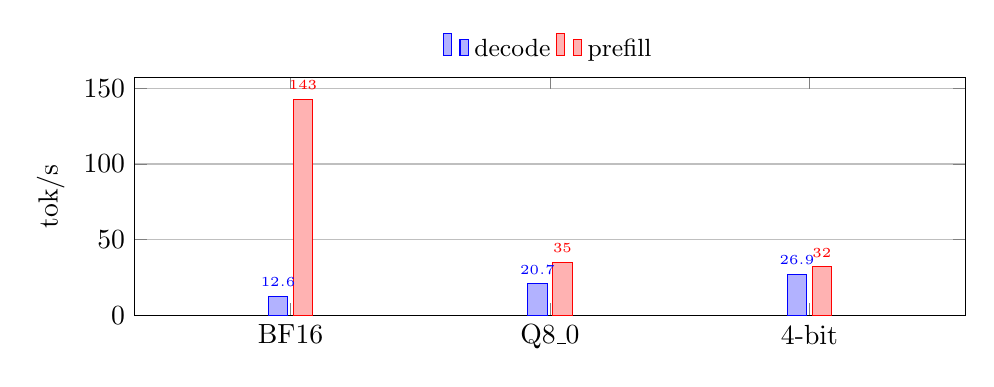
\begin{tikzpicture}
\begin{axis}[
  width=\columnwidth, height=4.6cm,
  ybar, bar width=7pt, ymin=0,
  ylabel={tok/s}, ymajorgrids, tick align=inside,
  symbolic x coords={BF16, Q8\_0, 4-bit},
  xtick=data, enlarge x limits=0.3,
  legend style={at={(0.5,1.02)}, anchor=south, legend columns=2,
                draw=none, font=\small},
  nodes near coords, every node near coord/.append style={font=\tiny},
]
\addplot coordinates {(BF16,12.6) (Q8\_0,20.7) (4-bit,26.9)};
\addplot coordinates {(BF16,143) (Q8\_0,35) (4-bit,32)};
\legend{decode, prefill}
\end{axis}
\end{tikzpicture}
\caption{The quantization trade-off (Qwen3-4B, M5 Metal). Quantization
lifts bandwidth-bound \emph{decode} but lowers compute-bound \emph{prefill},
which lacks a quantized matrix-multiply kernel.}
\label{fig:tradeoff}
\end{figure}

\paragraph{Speculative decoding.} \Cref{tab:spec} reports acceptance rate
$\alpha$, block efficiency (accepted tokens per target forward), and wall-clock
speedup across workloads. Prompt-lookup lifts copy-heavy decode from $21.7$ to
\SpecDecodeRep{}~tok/s ($\SpecSpeedupRep\times$) at $\alpha{=}1.0$, but
\emph{slows} code ($\SpecSpeedupCode\times$) and open-ended text
($\SpecSpeedupChat\times$). The reason is specific to a bandwidth-bound engine:
the $k{+}1$-token verify does not amortize weight streaming at small draft
batch, so each speculative step costs close to $k{+}1$ decodes while advancing
by only (accepted$+1$) tokens---a penalty that is \emph{harsher} than on
compute-bound engines when $\alpha$ is low. This motivates two improvements
(\Cref{sec:related}): a batched matrix-multiply verify kernel that amortizes
weights, and adaptive draft gating that stops drafting when recent acceptance
is low. Crucially, in every case the emitted tokens are identical to greedy
decoding---speculation never changes the output, only the wall clock.

\begin{table}[t]\centering\small
\caption{Prompt-lookup speculative decoding by workload (Qwen3-4B Q8\_0, M5),
controlled A/B, median of 3. Speedup ${<}1$ means slower than plain decode.}
\label{tab:spec}
\begin{tabular}{lrrr}
\toprule
Workload & $\alpha$ & Blk.\ eff. & Speedup \\
\midrule
Repetitive / copy-heavy & 1.00 & 4.00 & $\SpecSpeedupRep\times$ \\
Code                    & 0.17 & 1.39 & $\SpecSpeedupCode\times$ \\
Open-ended / grounded   & 0.04 & 1.10 & $\SpecSpeedupChat\times$ \\
\bottomrule
\end{tabular}
\end{table}

\paragraph{Memory.} Peak process RSS is $\sim$\PeakRSS{}~MB for the 4B model
regardless of quantization, since weights are \code{mmap}-ed and paged in on
demand; we report artifact size alongside RSS, as peak RSS understates true
residency for GPU-touched \code{mmap} pages.

\section{Related Work}
\label{sec:related}
\paragraph{Paged KV and relocation.} PagedAttention \citep{kwon2023pagedattention}
introduced the block table; SGLang's RadixAttention \citep{zheng2024sglang}
shares prefixes across calls via a radix tree. Both rely on placement- and
sharing-correctness and test throughput and cache-hit rate, not a
placement-permutation invariant. Systems that migrate KV blocks at runtime for
load balancing treat relocatability as safe by construction. Kipp instead makes
placement-invariance an explicit passing gate.

\paragraph{Determinism.} \citet{he2025defeating} trace run-to-run
nondeterminism to batch-size-dependent kernel reductions and restore bitwise
determinism with batch-invariant kernels, subsequently adopted for
deterministic serving. That work fixes the reduction-order axis; our contract
fixes the orthogonal spatial (physical-placement) axis and adds a byte-stable
scalar oracle as a hard cross-backend gate.

\paragraph{Attention and quantization.} FlashAttention
\citep{dao2022flashattention,dao2024flashattention2,shah2024flashattention3}
made exact attention IO-efficient; Kipp's streaming online-softmax Metal
kernel is in this lineage. Post-training quantization
\citep{frantar2023gptq,lin2024awq} and GGUF k-quants \citep{llamacpp2023gguf}
inform Kipp's block-quantized weights.

\paragraph{Speculative decoding.} Speculative decoding
\citep{leviathan2023speculative,chen2023speculativesampling} and its
draft-model-free \citep{saxena2023promptlookup} and self-drafting
\citep{cai2024medusa,li2024eagle,li2024eagle2} variants accelerate decode.
Chain methods roll back by cheap truncation; dense-buffer tree methods pay a
gather-copy. Extending Kipp's placement-invariance gate to \emph{tree}-shaped
speculative rollback---reclaiming rejected branches by block-table unlinking
with a bitwise-safety gate---is a promising direction the chain-only mainline
lacks.

\section{Limitations and Future Work}
Placement-invariance is claimed only for retained KV, not logical reordering or
prefill-column permutation (\Cref{sec:vpa}). CUDA paging and the cross-request
block pool are implemented but not yet wired into the serving path; CUDA is
gated for correctness on cloud A100s but throughput numbers are reported only
where measured. A quantized matrix-multiply prefill kernel would remove the
prefill regression of \Cref{tab:perf}. The most promising extension is
tree-speculative rollback under the same invariance gate.

\section{Conclusion}
Kipp shows that the placement-invariance every paged inference system relies on
can be a \emph{tested} contract rather than an assumption, and that a
byte-stable scalar oracle can hold real GPU backends to exact arg\,max. The
result is a small, fast, and---above all---continuously verifiable engine: not
the fastest, but one where correctness is reproducible by re-execution.

\balance
\bibliographystyle{plainnat}
\bibliography{references}

\end{document}
